\FloatBarrier
\section{Extended related work}\label{app:related}

\textbf{Audio-based hit prediction.} Pachet and Roy~\cite{pachet2008hit} found that
acoustic and human-annotated descriptors could not predict popularity, while Ni
et~al.~\cite{ni2011hit} and Herremans et~al.~\cite{herremans2014dance} reported
above-chance results on chart data. Yang et~al.~\cite{yang2017revisiting} revisited the
problem with convolutional networks on audio. Zangerle et~al.~\cite{zangerle2019hit}
combined low- and high-level Essentia descriptors~\cite{bogdanov2013essentia} of Million
Song Dataset tracks~\cite{bertinmahieux2011million} in a wide-and-deep network and reached
75.04\,\% accuracy on a balanced set of 11{,}664 songs (5{,}832 hits; one is lost to a missing year or
incomplete descriptors, so we keep 5{,}831, App.~\ref{app:data}), noting that adding the release year
improved every configuration.

\textbf{Artist reputation.} Interiano et~al.~\cite{interiano2018musical} analyse more
than 500{,}000 UK songs (1985--2015) and show that a superstar indicator improves the
prediction of chart success over acoustic features alone. Salganik
et~al.~\cite{salganik2006experimental} showed experimentally that success in cultural
markets depends on social influence and cumulative advantage, which is one reason why an
artist's past success predicts future success.

\textbf{Spotify descriptors and Billboard labels.} Middlebrook and
Sheik~\cite{middlebrook2019song} matched about 24{,}000 Spotify tracks (1985--2018) to the
Hot~100 and reported 87.7\,\% test accuracy with a Random Forest; their feature list
includes chart-derived fields and an artist past-performance feature. SpotHitPy~\cite{dimolitsas2023spothitpy}
reported about 86\,\% on roughly 18{,}500 songs. Zhao et~al.~\cite{zhao2023analysis}
added engineered metadata and lyrics features for Top-10 prediction (89.1\,\% with a
Random Forest). These numbers come from different datasets and label definitions.
The Spotify Hit Predictor dataset~\cite{ansari2020dataset} is a public benchmark of
decade-balanced hits and non-hits (1960--2019); the only academic study we found on it is
an MSc thesis by Du~\cite{du2022spotify}, which reports 84\,\% (2000s) and 82\,\% (2010s)
with one Random Forest per decade.

\textbf{Multimodal and popularity prediction.} Mart\'in-Guti\'errez
et~al.~\cite{martingutierrez2020multimodal} released SpotGenTrack and predicted Spotify
popularity with an end-to-end multimodal network; DeepHits~\cite{nofer2026deephits}
combines log-Mel CNNs, lyric embeddings, artist popularity and release year on the same
data; Rompolas et~al.~\cite{rompolas2024predicting} use social-media sentiment.

\textbf{Evaluation pitfalls.} Dietterich~\cite{dietterich1998approximate} recommends
McNemar's test for a single split, and Nadeau and Bengio~\cite{nadeau2003inference} show
that naive $t$-tests over overlapping resamples are anti-conservative and propose a
corrected variance. Leakage~\cite{kaufman2012leakage} and shortcut
learning~\cite{geirhos2020shortcut} describe models that exploit cues unrelated to the
intended task. In music information retrieval, Sturm~\cite{sturm2014simple} showed that
systems can reach high scores through confounds in the ground truth (``horses''), and
Flexer~\cite{flexer2007closer} showed that letting songs by the same artist appear in
training and test sets inflates genre-classification accuracy; our artist-grouped
cross-validation applies this artist filter to hit prediction. To our knowledge, no hit-prediction study on Spotify descriptors reports
both a significance-tested head-to-head on the same data and an audit of construction
artefacts.

\FloatBarrier
\section{Datasets in detail}\label{app:data}

\textbf{Spotify Hit Predictor.} Six decade files (1960s--2010s) list 13 Spotify audio
descriptors (danceability, energy, key, loudness, mode, speechiness, acousticness,
instrumentalness, liveness, valence, tempo, duration, time signature), two analysis
fields (\texttt{chorus\_hit}, \texttt{sections}), the artist, the title and a binary
target~\cite{ansari2020dataset}. The six files hold 41{,}106 rows; 537 track URIs (App.~\ref{app:glossary})
appear more than once, 450 of them in two decade files and 26 with different labels. We keep the first copy in the
order the files are read (00s, 10s, 60s, 70s, 80s, 90s, i.e.\ alphabetical), which leaves 40{,}560 songs; a
song's decade is the decade of the file that copy comes from. A song is a hit if it appeared on the weekly Hot~100 in that decade. Crucially,
the dataset documentation states that a non-hit must satisfy all of: the track is not in
that decade's hit list, \emph{its artist is not in that decade's hit list}, it belongs to a
``non-mainstream and/or avant-garde'' genre, and that genre has no song in the hit list.
Each decade file is therefore balanced (48.3--49.9\,\% hits), and the negative class is
selected partly \emph{by artist} and \emph{by genre}. We return to this in
Sec.~\ref{sec:discussion}.

\textbf{Audio subset.} We first drew a random sample of 3{,}996 songs, the same number (333) in each of
the 12 decade $\times$ hit/non-hit cells (seed 42), and searched each one on the public Deezer API with the
query \texttt{artist:"<artist>" track:"<title>"} (the raw artist and title fields of the dataset, with double quotes
and backslashes removed), keeping the 30-second preview of the first result (the
quoted fields make Deezer require both the artist and the title; the match is not checked further, so a few
previews may be another version of the song). 3{,}562 songs
had a preview and complete descriptors; this is the \emph{audio subset}. The same search was later run on every
song (35{,}370 found, App.~\ref{sec:audit}). From the previews we extracted 31 spectral/rhythmic descriptors (``FFT'') and 185 richer
librosa~\cite{mcfee2015librosa} descriptors (20 MFCCs and their first and second
derivatives, chroma, tonnetz, spectral contrast, centroid, bandwidth, roll-off, flatness,
zero-crossing rate, RMS and onset/tempogram statistics, each summarised by mean and
standard deviation).

\textbf{ISMIR 2019.} The release of Zangerle et~al.~\cite{zangerle2019hit} provides
Essentia low- and high-level descriptors for 5{,}832 Hot~100 hits and 89{,}235 non-hits
from the Million Song Dataset, in two files (\texttt{msd\_bb\_matches.csv}, \texttt{msd\_bb\_non\_matches.csv}) that
give for each track its MSD identifier, artist, title and release year (from the MSD metadata). Tracks with a
missing or zero year are removed. On ISMIR the artist name is only lower-cased and trimmed (no accent or
featuring removal). We flatten all numeric descriptors of the Essentia JSON files: numbers are kept, lists of
numbers are summarised by their mean, while booleans, strings, lists of lists, the whole \texttt{metadata} block
(bit rate, codec, \dots) and the beat positions in seconds are skipped; we then keep the columns present for more
than 95\,\% of the tracks (computed over all tracks with descriptors: the hits and the whole non-hit pool), giving 592, drop every track with a missing value in one of them (no imputation),
keep the 5{,}831 hits with complete
descriptors and, like the original study, draw an equal number of non-hits (protocol A, 11{,}662 songs). The
year-matched sample of protocol B also has 11{,}662 songs. Hits have a median release year of 1987 and non-hits of 2001, a fact that matters
below.

\textbf{SpotGenTrack.} 101{,}909 Spotify tracks with 13 descriptors, 207 pre-extracted
low-level audio features and a popularity score~\cite{martingutierrez2020multimodal}; we
label tracks with popularity $\geq 55$ as hits (19.4\,\%). Because the classes are
imbalanced, we report ROC-AUC alongside accuracy for this dataset.

A fourth candidate, a Billboard year-end chart file (2000--2023) augmented with Spotify
features, was discarded: 2{,}911 of its 3{,}397 rows have no audio descriptors.

\FloatBarrier
\section{Main result: more detail}\label{app:main}
\begin{table}[!htbp]
\centering
\caption{Cross-validated accuracy per decade: the models of Table~\ref{tab:main}, trained on all decades in each
of the 25 folds, scored separately on the test songs of each decade (Random Forest).}
\label{tab:decade}
\footnotesize
\setlength{\tabcolsep}{3.2pt}
\begin{adjustbox}{max width=\columnwidth}
\begin{tabular}{@{}lcccccc@{}}
\toprule
Features & 60s & 70s & 80s & 90s & 00s & 10s \\
\midrule
Audio (13) & .743 & .750 & .770 & .806 & .836 & .816 \\
+ decade & .764 & .763 & .794 & .840 & .851 & .833 \\
+ artist & .763 & .784 & .812 & .831 & .860 & .842 \\
+ decade + artist & \textbf{.788} & \textbf{.796} & \textbf{.836} & \textbf{.864} & \textbf{.873} & \textbf{.868} \\
\bottomrule
\end{tabular}
\end{adjustbox}
\end{table}

The improvement holds in every decade (Table~\ref{tab:decade}), from $+3.7$\pp{} in the
2000s to $+6.6$\pp{} in the 1980s. Since each decade file is balanced, the decade indicator
carries no information on its own; its gain can only come from interactions with the audio
descriptors, i.e.\ from era-specific decision rules.

\begin{table}[!htbp]
\centering
\caption{Robustness to the classifier (5-fold CV with one repeat, $5{\times}1$, corrected $t$-test; all 5 folds
improve).}
\label{tab:models}
\footnotesize
\setlength{\tabcolsep}{3pt}
\begin{adjustbox}{max width=\columnwidth}
\begin{tabular}{@{}lcccc@{}}
\toprule
Classifier & Audio (13) & + decade + artist & $\Delta$ & $p$ \\
\midrule
Random Forest~\cite{breiman2001random} & .780 & .832 & +5.2 & $2{\cdot}10^{-5}$ \\
XGBoost~\cite{chen2016xgboost} & .788 & \textbf{.845} & +5.7 & $3{\cdot}10^{-7}$ \\
Logistic regression & .727 & .782 & +5.5 & $4{\cdot}10^{-5}$ \\
$k$-NN ($k=25$) & .750 & .796 & +4.6 & $8{\cdot}10^{-6}$ \\
SVM (RBF) & .773 & .828 & +5.5 & $3{\cdot}10^{-5}$ \\
\bottomrule
\end{tabular}
\end{adjustbox}
\end{table}

\textbf{Robustness to the classifier.} The gain is of the same size for five classifiers of
very different nature (Table~\ref{tab:models}), so it comes from the features rather than
from the model. XGBoost is the strongest on average, but on the canonical split it ties with
the frozen Random Forest (0.820 vs 0.822, McNemar $p=0.87$). TreeSHAP attributions of the
XGBoost model rank artist history first (mean $|\phi|=1.08$), the six decade indicators
second (0.86 summed) and instrumentalness third (0.73), ahead of every other descriptor.

\textbf{Future decades.} To test whether the gain survives a temporal shift, we train on all
earlier decades and test on a later one, with no song from the test decade seen in
training: 1960s--80s $\to$ 1990s, 1960s--90s $\to$ 2000s, 1960s--2000s $\to$ 2010s (we start at the 1990s so that
the training set always spans at least three decades). Artist history improves the Random Forest by $+2.5$\pp{} on the 1990s
(0.736 $\to$ 0.761), $+1.9$\pp{} on the 2000s (0.805 $\to$ 0.824) and $+3.4$\pp{} on the
2010s (0.780 $\to$ 0.814; McNemar $p$ between $10^{-7}$ and $10^{-21}$), with similar gains
for XGBoost. The decade indicator cannot be used here, since the test decade never
appears in training.


\FloatBarrier
\section{Where the accuracy comes from: PCA and everything together}\label{app:ablation}
\textbf{Which descriptors matter: PCA.} To see which of the 13 Spotify descriptors carry the
signal, we ran a principal component analysis on the standardised descriptors
(Fig.~\ref{fig:pca}). The first component (23.6\,\% of the variance) is an \emph{intensity} axis
(energy $+0.48$, loudness $+0.47$, acousticness $-0.43$) and is also the one that best separates hits
(ROC-AUC 0.70 on its own). The second (11.1\,\%) is a \emph{mood} axis (danceability $+0.48$,
valence $+0.44$, duration $-0.36$; AUC 0.62). The next four components together explain another
33\,\% of the variance but separate hits no better than chance (AUC 0.50--0.52), and eight components
are needed to reach 81\,\%. Variance and usefulness therefore do not coincide. Among single descriptors,
the most separating are instrumentalness (AUC 0.74, lower in hits), danceability (0.70, higher),
loudness (0.64) and valence (0.64); key, duration and tempo are close to chance (0.51--0.52). Replacing
the descriptors by their components only loses accuracy: the frozen Random Forest reaches 0.575 with
one component, 0.710 with six and 0.765 with all 13, against 0.782 for the raw descriptors ($-1.7$\pp{}
even though no information is removed, 0/25 folds, $p=2\times10^{-8}$). Trees split on one input at a
time, and rotating the axes mixes a sparse, highly informative descriptor (instrumentalness) into
components shared with uninformative ones. We therefore keep the raw descriptors; PCA is used only for the
185-dimensional librosa representation (App.~\ref{sec:audit}).

\begin{figure*}[t]
\centering
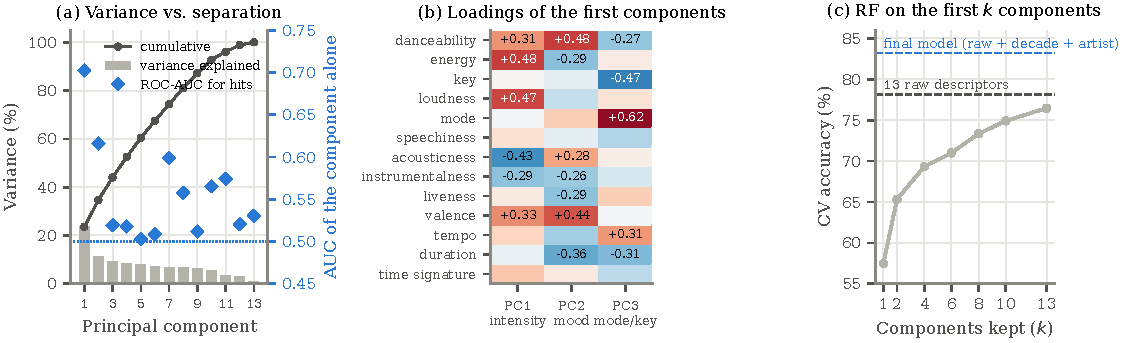
\includegraphics[width=\textwidth]{fig_pca.pdf}
\caption{PCA of the 13 Spotify descriptors (40{,}560 songs). (a) Variance explained by each component
(bars), cumulative (line), and how well each component alone separates hits from non-hits (ROC-AUC, right
axis; dotted line = chance). (b) Loadings of the first three components (values below 0.25 in absolute
value are not printed). (c) Cross-validated accuracy of the frozen Random Forest trained on the first $k$
components, against the 13 raw descriptors and the final model.}
\label{fig:pca}
\end{figure*}

\textbf{Training on everything at once.} One might simply put every input we built into one model. We did
this on the 35{,}370 songs that have a preview (needed for FFT), with the same frozen Random Forest and
$5{\times}5$ CV (Table~\ref{tab:all}). The full model reaches 0.883, 5.8 points above the final model
(0.825 on these songs). That gain does not come from music. Removing the song title alone takes it down to
0.843 ($-4.0$\pp, $p=3\times10^{-19}$), and the title is an artefact of how the non-hits were collected
(App.~\ref{sec:audit}). The remaining $+1.8$\pp{} over the final model must come, by elimination, from FFT and
the market-trend features, the only other blocks that matter (removing either one costs $-0.4$ and $-0.3$\pp; title
length and \texttt{chorus\_hit}/\texttt{sections} change nothing; the two overlap, so each costs less alone), whose gains vanish under the genre control and carry
only the era (App.~\ref{sec:further} and Sec.~\ref{sec:timeseries}). Once FFT and trend are in, the decade
indicators become redundant ($-0.2$\pp, $p=0.11$): all three describe the era. Artist history remains the
input whose removal costs the most among the legitimate ones ($-1.9$\pp, $p=2\times10^{-11}$), ahead of
the 13 descriptors ($-1.2$\pp), while \texttt{chorus\_hit}/\texttt{sections} and title length change nothing.
Training on everything therefore gives a higher number on this benchmark by learning how it was built. The
model we keep is the one whose inputs survive the controls: the 20 inputs of the final model.

\begin{table}[!htbp]
\centering
\caption{Training on every input at once (35{,}370 songs with a preview, frozen Random Forest, $5{\times}5$
CV). Left: one block removed from ``everything'' ($\Delta$ vs everything). Right: the block alone.
$^{*}$Decade alone scores .532 here, not the .503 of the full benchmark, because these songs are 53.2\,\% hits: the
decade carries no information and the model predicts the majority class.}
\label{tab:all}
\footnotesize
\setlength{\tabcolsep}{3pt}
\begin{adjustbox}{max width=\columnwidth}
\begin{tabular}{@{}lccc@{}}
\toprule
Model & Acc. & AUC & $\Delta$ ($p$) \\
\midrule
Final model (Spotify + decade + artist) & .825 & .911 & -- \\
Everything (8 blocks) & \textbf{.883} & .952 & +5.8 ($3{\cdot}10^{-21}$) vs final \\
Everything except song title & .843 & .925 & +1.8 ($6{\cdot}10^{-10}$) vs final \\
\midrule
\multicolumn{4}{@{}l}{\emph{Remove one block from everything}} \\
\quad $-$ song title & .843 & .925 & $-4.0$ ($3{\cdot}10^{-19}$) \\
\quad $-$ artist history & .864 & .933 & $-1.9$ ($2{\cdot}10^{-11}$) \\
\quad $-$ Spotify (13) & .871 & .944 & $-1.2$ ($5{\cdot}10^{-8}$) \\
\quad $-$ FFT (31) & .879 & .949 & $-0.4$ (.01) \\
\quad $-$ market trend (2) & .879 & .949 & $-0.3$ (.01) \\
\quad $-$ decade (6) & .881 & .950 & $-0.2$ (.11) \\
\quad $-$ title length & .883 & .951 & $-0.0$ (.93) \\
\quad $-$ chorus\_hit + sections & .883 & .952 & $+0.0$ (.75) \\
\midrule
\multicolumn{4}{@{}l}{\emph{One block alone}} \\
\quad Spotify (13) / FFT (31) & .777 / .773 & .849 / .847 & -- \\
\quad artist history / song title & .648 / .660 & .669 / .740 & -- \\
\quad market trend / title length & .629 / .546 & .672 / .545 & -- \\
\quad chorus\_hit + sections / decade & .543 / .532$^{*}$ & .563 / .516 & -- \\
\bottomrule
\end{tabular}
\end{adjustbox}
\end{table}

\FloatBarrier
\section{Head-to-head with Du: table}\label{app:tilburg}
\begin{table}[!htbp]
\centering
\caption{Head-to-head with Du~\cite{du2022spotify} using their protocol (one model per
decade, 13 audio + \texttt{chorus\_hit} + \texttt{sections}, 70/30 split) over 50 random
splits: mean accuracy (std). RF: Random Forest; LR: logistic regression; cfg.: configuration. ``Wins'' counts
splits where adding artist history helps; $p$: corrected $t$-test over the $J=50$ paired splits,
$n_{\text{test}}/n_{\text{train}}=3/7$.}
\label{tab:tilburg}
\footnotesize
\setlength{\tabcolsep}{2.6pt}
\begin{adjustbox}{max width=\columnwidth}
\begin{tabular}{@{}llcccc@{}}
\toprule
Dec. & Model & Published & Re-impl. & + artist & Wins / $p$ \\
\midrule
\multirow{3}{*}{00s} & RF (their cfg.) & .84 & .846 (.009) & \textbf{.867} (.009) & 50 / $9{\cdot}10^{-8}$ \\
& LR (their cfg.) & .82 & .821 (.007) & \textbf{.848} (.007) & 50 / $2{\cdot}10^{-9}$ \\
& RF (frozen) & -- & .852 (.008) & \textbf{.875} (.006) & 50 / $10^{-7}$ \\
\midrule
\multirow{3}{*}{10s} & RF (their cfg.) & .82 & .829 (.008) & \textbf{.861} (.008) & 50 / $4{\cdot}10^{-11}$ \\
& LR (their cfg.) & .79 & .807 (.009) & \textbf{.835} (.008) & 50 / $6{\cdot}10^{-6}$ \\
& RF (frozen) & -- & .841 (.008) & \textbf{.873} (.008) & 50 / $9{\cdot}10^{-10}$ \\
\bottomrule
\end{tabular}
\end{adjustbox}
\end{table}

\FloatBarrier
\section{External validation: more detail}\label{app:external}

\begin{figure}[!htbp]
\centering
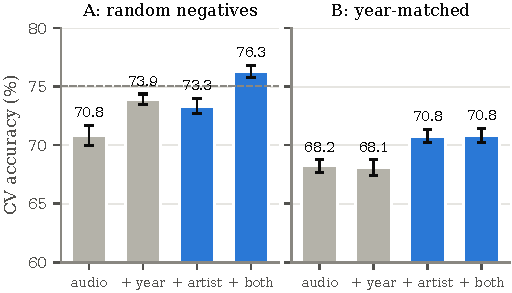
\includegraphics[width=\columnwidth]{fig_ismir.pdf}
\caption{ISMIR 2019 data, cross-validated accuracy with 95\,\% CI. Gray: without artist
history; blue: with it (``both'' = year + artist). Dashed line in A: best published
accuracy~\cite{zangerle2019hit}. Matching years (B) removes the gain of release year but not
that of artist history.}
\label{fig:ismir}
\end{figure}

\begin{table}[!htbp]
\centering
\caption{SpotGenTrack (101{,}909 tracks, 19.4\,\% hits; always predicting ``non-hit''
scores 0.806). 5-fold CV, corrected $t$-test vs the 13 descriptors.}
\label{tab:sgt}
\footnotesize
\setlength{\tabcolsep}{3pt}
\begin{adjustbox}{max width=\columnwidth}
\begin{tabular}{@{}lccc@{}}
\toprule
Features & Acc. [95\,\% CI] & ROC-AUC & $p$ (acc.) \\
\midrule
Spotify descriptors (13) & .812 [.811,.813] & .690 & -- \\
+ decade & .812 [.811,.813] & .712 & .66 \\
+ artist & .823 [.821,.826] & .762 & $10^{-3}$ \\
\textbf{+ decade + artist} & \textbf{.825} [.823,.827] & \textbf{.777} & $3{\cdot}10^{-4}$ \\
+ artist + low-level audio & .825 [.823,.828] & .758 & $2{\cdot}10^{-4}$ \\
\bottomrule
\end{tabular}
\end{adjustbox}
\end{table}

\textbf{SpotGenTrack.} Here the label is Spotify popularity rather than a chart, and
80.6\,\% of tracks are negatives, so accuracy is dominated by the majority class: the 13
descriptors score 0.812, barely above always predicting ``non-hit''. Ranking quality tells
the real story (Table~\ref{tab:sgt}): artist history raises ROC-AUC from 0.690 to 0.762
($+7.2$ points), and with decade to 0.777. On the hit class, the 13 descriptors find
only 8.3\,\% of the hits (F1 0.147); with decade and artist history, recall rises to
25.2\,\% at unchanged precision (0.62) and F1 to 0.358 (5/5 folds, $p=7\times10^{-7}$),
while the 207 low-level audio features add
nothing on top of artist history. A single 75/25 split gives the same picture (accuracy
0.810 $\to$ 0.822 and ROC-AUC 0.688 $\to$ 0.760 with artist history, McNemar
$p=6\times10^{-13}$).


\FloatBarrier
\section{Unseen artists and cold start: table}\label{app:robust}
\begin{table}[!htbp]
\centering
\caption{Robustness. Top: cross-validated accuracy with random stratified folds vs folds
grouped by artist (no test artist seen in training). Era = decade (Hit Predictor) or
release year (ISMIR). Bottom: gain over audio in grouped CV, on songs whose artist had no
earlier hit (new) or at least one (known). New/known songs: 33{,}438/7{,}122 (Hit
Predictor), 7{,}480/4{,}182 (ISMIR A), 7{,}269/4{,}393 (ISMIR B). The accuracy on each group is computed inside
each test fold; the corrected $t$-test uses the per-fold differences on that group and the ratio
$n_{\text{test}}/n_{\text{train}}$ of the whole fold.}
\label{tab:robust}
\footnotesize
\setlength{\tabcolsep}{2.6pt}
\begin{adjustbox}{max width=\columnwidth}
\begin{tabular}{@{}llcccc@{}}
\toprule
Data & Folds & Audio & + era & + artist & + both \\
\midrule
\multirow{2}{*}{Hit Predictor} & random & .782 & .802 & .810 & .832 \\
 & by artist & .772 & .792 & .802 & \textbf{.822} \\
\multirow{2}{*}{ISMIR A} & random & .708 & .739 & .733 & .763 \\
 & by artist & .709 & .739 & .730 & \textbf{.759} \\
\multirow{2}{*}{ISMIR B} & random & .682 & .681 & .708 & .708 \\
 & by artist & .677 & .678 & \textbf{.705} & \textbf{.705} \\
\midrule
& Hits (\%) & \multicolumn{2}{c}{New artists: $\Delta$ ($p$)} & \multicolumn{2}{c}{Known: $\Delta$ ($p$)} \\
\cmidrule(lr){3-4}\cmidrule(l){5-6}
& new/known & + era & + artist & \multicolumn{2}{c}{+ artist} \\
\midrule
Hit Predictor & 39 / 97 & +2.2 ($2{\cdot}10^{-9}$) & +0.4 (.17) & \multicolumn{2}{c}{+15.0 ($3{\cdot}10^{-14}$)} \\
ISMIR A & 36 / 75 & +3.4 ($6{\cdot}10^{-5}$) & +0.8 (.08) & \multicolumn{2}{c}{+4.4 (.003)} \\
ISMIR B & 37 / 72 & +0.1 (.79) & +1.4 (.002) & \multicolumn{2}{c}{+5.3 ($8{\cdot}10^{-5}$)} \\
\bottomrule
\end{tabular}
\end{adjustbox}
\end{table}

\textbf{Artist-grouped cross-validation.} With random folds, songs by the same artist can
fall in both the training and the test part, so a model could recognise an artist from the
audio. We therefore repeat every protocol with stratified group $k$-fold, grouping songs by
normalised artist so that no test artist is seen in training (Table~\ref{tab:robust}, top).
Accuracies drop by up to one point, a small artist-identity effect in the audio
descriptors, but the gains remain: $+5.0$\pp{} for decade and artist on the Hit
Predictor (unchanged, 25/25 folds, $p=10^{-13}$) and $+2.9$\pp{} for artist history in the
year-matched ISMIR protocol (10/10, $p=9\times10^{-7}$). In protocol A the gains lose at
most half a point, and audio, year and artist still reach 0.759 [0.752, 0.766], above the
published 75.04\,\%.

\textbf{Cold start.} Table~\ref{tab:robust} (bottom) splits the grouped test folds by
whether the artist had an earlier hit. On the Hit Predictor, artist history does not help
new artists ($+0.4$\pp, $p=0.17$): its whole gain comes from the 17.6\,\% of songs by
established artists, 96.6\,\% of which are hits, which quantifies the benchmark effect
discussed in Sec.~\ref{sec:discussion}. The decade, in contrast, helps new artists
($+2.2$\pp, $p=2\times10^{-9}$). On ISMIR, where songs by established artists are hits
only 72--75\,\% of the time, artist history also tends to help new artists in the year-matched
protocol ($+1.4$\pp, $p=0.002$, 10/10 folds; above the Bonferroni threshold, so indicative only), perhaps
because an empty history is itself informative when negatives are not selected by artist. On ISMIR, ``new''
means no earlier hit among the dataset's own hits (the reference set there), not in the whole Hot~100.


\FloatBarrier
\section{Audit and further experiments}\label{app:audit}\label{sec:audit}\label{sec:further}
\begin{table}[!htbp]
\centering
\caption{Audit of candidate gains. Single split (McNemar) vs $5{\times}5$ cross-validation
(corrected $t$-test). Top: full benchmark (single split = the canonical split, 2{,}000 test songs). Bottom:
3{,}562-song audio subset (single split = its stratified 75/25 split, 891 test songs).}
\label{tab:audit}
\footnotesize
\setlength{\tabcolsep}{2.6pt}
\begin{adjustbox}{max width=\columnwidth}
\begin{tabular}{@{}lcccl@{}}
\toprule
Added to audio & Split $\Delta$ ($p$) & CV $\Delta$ & CV $p$ & Verdict \\
\midrule
Song title (TF-IDF) & +6.9 ($4{\cdot}10^{-14}$) & +6.7 & $4{\cdot}10^{-20}$ & artefact \\
\texttt{chorus\_hit}+\texttt{sections} & +0.6 (.32) & $-$0.0 & .82 & no effect \\
Title length & +0.05 (1.0) & +0.2 & .28 & no effect \\
\midrule
Rich librosa (PCA 40) & +3.8 (.002) & +0.9 & .15 & not significant \\
FFT descriptors (31) & +4.4 (.001) & +2.3 & .007 & small \\
Decade & +1.1 (.27) & +1.0 & .03 & small \\
Artist & +3.4 (.010) & +3.8 & $2{\cdot}10^{-6}$ & robust \\
Artist + rich & +6.7 ($10^{-6}$) & +4.9 & $10^{-8}$ & = artist \\
Decade + artist & +3.6 (.006) & +5.1 & $10^{-8}$ & robust \\
\bottomrule
\end{tabular}
\end{adjustbox}
\end{table}

\textbf{Titles.} A title model trained out-of-fold adds $+6.7$\pp, more than any musical
feature. Its largest weights show why. On the non-hit side: \emph{remastered, feat, live, version, remix, mix,
edit, demo, mono, medley}, genre words (\emph{blues, metal, ambient, punk, rock, death, jazz, hardcore}) and
non-English words (\emph{remasterizado, de, te, en}); on the hit side: ordinary words (\emph{nights, you, party,
kiss, love, sunshine}). On the genre-matched sample of App.~\ref{sec:further} (7{,}554 songs), 13.5\,\% of the
non-hit titles contain `` - '' (a Spotify suffix such as ``- Remastered 2011''), against 0.1\,\% of the hits;
5.7\,\% contain ``remaster'' (hits: 0), and 5.7\,\% contain non-ASCII letters (hits: 0.1\,\%). The hit titles have
evidently been cleaned and the non-hit titles have not. We test this directly (\texttt{r8\_future\_work.py title},
$5{\times}5$ CV on the genre-matched sample). The title adds $+4.8$\pp{} to the 13 descriptors and $+2.9$\pp{} to
the final model (25/25, $p=2\times10^{-6}$), so genre explains only part of it. We then strip everything after
`` - '', anything in brackets and ``feat./ft./featuring \dots'' (this changes 19.0\,\% of non-hit titles and 4.9\,\%
of hit titles). The gain over the final model falls to $+1.9$\pp{} (23/25, $p=0.002$), above the Bonferroni
threshold. What remains is mostly genre and language vocabulary. We reject the title: its gain comes from how the
two classes were written down and collected, not from anything that makes a song a hit.

\textbf{Single split vs cross-validation.} On the small audio subset, the 185 rich librosa
descriptors appeared to add $+3.8$\pp{} with $p=0.002$ on the subset's single 75/25 split, but the
cross-validated gain is $+0.9$\pp{} and is not significant. The same holds for the choice
of the PCA dimension (5 to 100 components are within noise) and for the knock-out of any
descriptor family (all within $\pm0.1$\pp). In a block ablation of the full subset model,
only removing artist history causes a significant drop ($-3.3$\pp, $p=10^{-5}$). The
\texttt{chorus\_hit} and \texttt{sections} fields, often suspected of leakage, add nothing.

\textbf{FFT and the best audio-subset model.} The 31 FFT descriptors are the only extra
audio representation whose gain survives cross-validation, and it persists on top of
artist history: audio + artist + FFT reaches $0.821$ against $0.801$ for audio + artist
($+2.0$\pp, 23/25 folds, $p=0.008$). Adding decade to that model gives the best subset
accuracy, $0.824$, but the increment is not significant ($+0.3$\pp, $p=0.50$), and
decade adds nothing to FFT alone ($0.785$ with decade vs $0.786$ without): the spectral descriptors already
carry the era. Conversely, artist history still adds $+3.5$\pp{} on top of FFT
($p=4\times10^{-5}$). Fig.~\ref{fig:subset} shows every configuration we evaluated on
this subset.

\textbf{FFT on the whole benchmark.} We then retrieved Deezer previews for every song we
could match: 35{,}370 of the 40{,}560 songs (87.2\,\%). Deezer finds hits more often than
flops (94.0\,\% vs 80.6\,\%), so the covered set is 53.2\,\% hits and every comparison
below uses the same 35{,}370 songs. With $5{\times}5$ cross-validation, adding FFT to the
main model (audio + decade + artist) raises accuracy from $0.825$ to $0.839$ ($+1.4$\pp,
25/25 folds, $p=4\times10^{-9}$; AUC $0.911\to0.921$). The whole gain comes from songs by
new artists, $0.789\to0.807$ ($+1.8$\pp, 25/25, $p=6\times10^{-9}$), while songs by known
artists stay at $0.977$ ($-0.1$\pp, n.s.). Unlike on the small subset, decade remains
useful once FFT is present: audio + artist + FFT reaches only $0.829$ ($+0.4$\pp{} over the
main model, $p=0.04$). FFT thus appears to address the cold-start weakness of artist
history, but the benchmark's flops come from non-mainstream genres by construction, and
spectral descriptors can recognise genre. App.~\ref{sec:further} shows that this gain does
not survive a genre control.

\begin{figure}[!htbp]
\centering
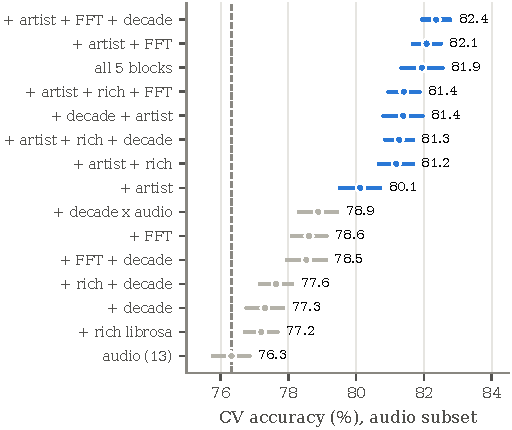
\includegraphics[width=\columnwidth]{fig_subset.pdf}
\caption{Every configuration evaluated on the 3{,}562-song audio subset, $5{\times}5$
cross-validated accuracy with 95\,\% CI, sorted. Blue: with artist history; gray: without.
Dashed line: the 13 Spotify descriptors alone. ``rich'': the 185 librosa descriptors (PCA 40); ``decade x
audio'': each of the 13 descriptors multiplied by each of the 6 decade indicators (78 inputs); ``all 5 blocks'':
audio + artist + decade + decade x audio + rich.}
\label{fig:subset}
\end{figure}


\textbf{Genre control for FFT.} We attach Spotify artist genres from the SpotGenTrack
release~\cite{martingutierrez2020multimodal} by normalised artist name (20{,}610 songs
with both a preview and a genre) and map the tags to 16 families. The benchmark's
construction is plainly visible: Latin, classical, jazz, ``world'' and metal artists
account for 50\,\% of the flops and 1.9\,\% of the hits, while rock, pop, R\&B,
hip-hop and country account for 93\,\% of the hits. Genre is also partly audible: a
Random Forest (200 trees, stratified shuffled 5-fold cross-validated predictions, seed 42) recovers the dominant
family from the 13 Spotify descriptors with 47.4\,\% accuracy,
from the 31 FFT descriptors with 49.9\,\% and from both with 53.3\,\% (majority class
26.1\,\%). Three results follow (Table~\ref{tab:genre}). (a) Genre families as features
raise the main model from $0.828$ to $0.928$ ($+10.1$\pp, 25/25, $p=8\times10^{-23}$):
on this benchmark, knowing the artist's genre is worth more than any audio
representation. (b) Once genre is known, FFT \emph{lowers} accuracy ($-1.1$\pp, 0/25,
$p=5\times10^{-7}$), also for new artists ($-1.4$\pp). (c) On a genre-matched sample
(as many hits as flops inside every family; 7{,}554 songs), FFT adds nothing to the main
model ($+0.1$\pp, 13/25, $p=0.84$; new artists $+0.1$\pp, $p=0.80$). FFT still improves
the 13 Spotify descriptors alone on that sample ($+2.5$\pp, 25/25, $p=5\times10^{-4}$),
but the main model, without FFT, still beats audio + FFT by $4.3$\pp{}
($p=2\times10^{-8}$), and decade and artist history add $+6.7$\pp{} to the 13 descriptors on that sample
(0.722 $\to$ 0.790, 25/25, $p=9\times10^{-13}$); each one alone also helps on that sample (decade $+2.5$\pp,
$p=8\times10^{-7}$; artist history $+4.2$\pp, $p=2\times10^{-8}$; \texttt{r8\_future\_work.py decadegenre}). We conclude that the full-benchmark FFT gain is a genre shortcut,
whereas the gain of artist history survives the genre control. Spotify assigns artist
genres retrospectively, so we use them only as a control, never as a predictive feature.

\begin{table}[!htbp]
\centering
\caption{Genre control for FFT ($5{\times}5$ CV). Left: songs with a preview and a Spotify
genre. Right: genre-matched sample. Accuracy overall and on songs by new artists.}
\label{tab:genre}
\setlength{\tabcolsep}{3pt}
\begin{tabular}{lcccc}
\toprule
& \multicolumn{2}{c}{All (20{,}610)} & \multicolumn{2}{c}{Matched (7{,}554)} \\
Model & Acc. & new art. & Acc. & new art. \\
\midrule
audio (13 descriptors) & -- & -- & .722 & -- \\
main (audio+decade+artist) & .828 & .780 & .790 & .749 \\
\quad + FFT & .841 & .798 & .791 & .750 \\
\quad + genre & .928 & .911 & -- & -- \\
\quad + genre + FFT & .917 & .897 & -- & -- \\
\midrule
decade vs audio, $\Delta$ ($p$) & \multicolumn{2}{c}{--} & \multicolumn{2}{c}{$+2.5$ ($8{\cdot}10^{-7}$)} \\
artist vs audio, $\Delta$ ($p$) & \multicolumn{2}{c}{--} & \multicolumn{2}{c}{$+4.2$ ($2{\cdot}10^{-8}$)} \\
main vs audio, $\Delta$ ($p$) & \multicolumn{2}{c}{--} & \multicolumn{2}{c}{$+6.7$ ($9{\cdot}10^{-13}$)} \\
FFT vs main, $\Delta$ ($p$) & \multicolumn{2}{c}{$+1.3$ ($1.1{\cdot}10^{-4}$)} & \multicolumn{2}{c}{$+0.1$ (.84)} \\
FFT vs main+genre, $\Delta$ ($p$) & \multicolumn{2}{c}{$-1.1$ ($5{\cdot}10^{-7}$)} & \multicolumn{2}{c}{--} \\
\bottomrule
\end{tabular}
\end{table}

\textbf{Artist resolution.} The 52.1\,\% match rate is not a matching problem: 99.99\,\%
of the hits have an artist found in the chart history (by construction, at the latest in their own decade),
against 5.4\,\% of the flops, and only 2.7\,\% of the flops have an artist who charted up to and including their
own decade (only about 1.2\,\% charted in an \emph{earlier} decade, i.e.\ have $h(s)>0$). The remaining
$\approx$1.5\,\% of flops have an artist whose normalised name has a Hot~100 entry in the flop's own decade,
although the dataset's rule excludes such artists: these are homonyms merged by our name matching, or chart
entries missing from the dataset's own hit list; they do not enter $h(s)$, which counts earlier decades only.
The unmatched songs are flops whose artists never charted. Two alternatives give
no gain: matching the full credited name before the primary artist (``Simon \&
Garfunkel'' rather than ``Simon'') lowers accuracy ($0.827$ vs $0.832$, $-0.5$\pp,
$p=4\times10^{-4}$), and crediting featured appearances changes nothing ($+0.1$\pp,
$p=0.39$). Canonical identifiers would avoid homonyms but cannot raise the match rate.

\textbf{How fast does a model age?} We train on a single decade and test on every later
one (Table~\ref{tab:decay}, songs with a preview). Audio-only accuracy falls from
$0.809$ within a decade to $0.765$ one decade later and $0.689$ three decades later.
Artist history slows the decay, and its advantage grows with the gap ($+2.8$\pp{} within
a decade, $+5.1$\pp{} three decades later). FFT behaves in the opposite way: it helps
within a decade ($+2.2$\pp) but hurts from three decades on, consistent with descriptors
that encode era-specific production and genre rather than lasting appeal. The cells
average 6 to 1 train/test pairs and are not tested for significance.

\begin{table}[!htbp]
\centering
\caption{Model ageing: train on one decade, test $k$ decades later (frozen Random Forest of the main model, one fit
per pair,
35{,}370 songs with a preview; $k=0$: 5-fold CV inside each decade). Mean accuracy over
the available decade pairs.}
\label{tab:decay}
\setlength{\tabcolsep}{4pt}
\begin{tabular}{cccccc}
\toprule
$k$ & pairs & audio & + artist & + FFT & + artist + FFT \\
\midrule
0 & 6 & .809 & .837 & .831 & \textbf{.859} \\
1 & 5 & .765 & .796 & .782 & \textbf{.810} \\
2 & 4 & .728 & \textbf{.775} & .736 & \textbf{.775} \\
3 & 3 & .689 & \textbf{.740} & .673 & .728 \\
4 & 2 & .666 & \textbf{.734} & .661 & .718 \\
5 & 1 & .664 & \textbf{.754} & .599 & .706 \\
\bottomrule
\end{tabular}
\end{table}

\textbf{Lyrics on SpotGenTrack.} SpotGenTrack provides six lexical descriptors of the lyrics (syllables
per word, words per sentence, sentence count, word count, sentence similarity,
vocabulary richness) for 79{,}420 tracks with lyrics (21.5\,\% hits; $5{\times}1$ CV as in
Sec.~\ref{sec:external}). They improve the 13 Spotify descriptors (AUC $0.678\to0.729$,
$p=3\times10^{-4}$) and still add on top of decade and artist history (accuracy
$0.808\to0.814$, 5/5 folds, $p=0.002$; AUC $0.774\to0.797$, $p=2\times10^{-5}$). The gain
is modest in accuracy because of the class imbalance, and such a small gain measured on five folds does not
survive the Bonferroni correction, so we tested lyrics again on a larger, balanced dataset.


\FloatBarrier
\section{Lyrics on ISMIR: more detail}\label{app:lyrics}
ISMIR songs are Million Song Dataset tracks (joined to the lyrics by their MSD track identifier), for which the official musiXmatch
release~\cite{bertinmahieux2011million} gives the lyrics of 237{,}662 tracks as word counts over the
5{,}000 most frequent (stemmed) words. Coverage is itself a shortcut: 56\,\% of the hits have lyrics against
36\,\% of the non-hit pool, so ``has lyrics'' would predict the label. We therefore keep only songs
\emph{with} lyrics on both sides and redraw balanced samples under protocols A and B. A second shortcut is
language: 97.5\,\% of the hits but only 80.5\,\% of the non-hits are mainly in English (at least 25\,\% of
their words among the 29 most common English words). We therefore also repeat every test on English songs
only: the non-English songs are removed first, and the balanced (protocol A) or year-matched (protocol B) sample is
then drawn again from what remains. Two lyrics inputs are added to the final ISMIR model (audio + year + artist history): eight lexical
features (log number of words and of distinct words, richness, repetition, share of \emph{I/me/my},
\emph{you/your}, \emph{love} and of common English words), and one bag-of-words score, the out-of-fold
probability of a TF-IDF logistic regression trained inside each training fold, as for titles.

\begin{table}[!htbp]
\centering
\caption{Lyrics on ISMIR 2019 (songs with lyrics only; Random Forest, $5{\times}2$ CV, corrected $t$-test
vs the final model of the same row; all rows 10/10 folds improved). Unseen: no artist in both training and
test folds.}
\label{tab:lyrics}
\footnotesize
\setlength{\tabcolsep}{2.6pt}
\begin{adjustbox}{max width=\columnwidth}
\begin{tabular}{@{}lccccc@{}}
\toprule
Sample & Songs & Final & + lyrics & $\Delta$ ($p$) & AUC \\
\midrule
A: random & 6{,}526 & .728 & \textbf{.775} & +4.7 ($3{\cdot}10^{-4}$) & .798$\to$.851 \\
B: year-matched & 6{,}478 & .676 & \textbf{.727} & +5.1 ($2{\cdot}10^{-5}$) & .732$\to$.802 \\
A, English & 6{,}364 & .718 & \textbf{.745} & +2.7 ($6{\cdot}10^{-4}$) & .788$\to$.820 \\
B, English & 6{,}294 & .658 & \textbf{.708} & +4.9 ($1.1{\cdot}10^{-4}$) & .720$\to$.772 \\
A, English, unseen & 6{,}364 & .712 & \textbf{.742} & +3.0 ($6{\cdot}10^{-4}$) & .785$\to$.817 \\
B, English, unseen & 6{,}294 & .656 & \textbf{.700} & +4.4 ($3{\cdot}10^{-5}$) & .717$\to$.764 \\
\midrule
\multicolumn{6}{@{}l}{Lyrics alone (the 8 lexical features + bag-of-words score, no audio, year or artist; B, year-matched): .702,} \\
\multicolumn{6}{@{}l}{above the final model without lyrics (.676). Artist history uses all ISMIR hits as reference set.} \\
\bottomrule
\end{tabular}
\end{adjustbox}
\end{table}

Table~\ref{tab:lyrics} and Fig.~\ref{fig:lyrics}a show that lyrics add $+4.7$ points in protocol~A and
$+5.1$ in the year-matched protocol~B, in all 10 folds. The gain shrinks but remains when only English songs are
kept ($+2.7$ and $+4.9$), and it remains when, in addition, no artist appears in both training and test folds
($+3.0$ and $+4.4$, $p=3\times10^{-5}$; AUC $+0.047$, $p=10^{-6}$), so it does not come from recognising the
vocabulary of artists seen in training. In the strictest setting (year-matched, English, unseen artists) the gain
survives the Bonferroni correction ($p=3\times10^{-5}<1.25\times10^{-4}$), as do the other protocol-B rows; the
three protocol-A rows ($p=3\times10^{-4}$ to $6\times10^{-4}$) do not, and are indicative only. In the year-matched
protocol, lyrics alone (0.702) are more accurate than audio, year and artist history together (0.676).
Fig.~\ref{fig:lyrics}b shows what the model reads. Hit lyrics favour \emph{love} (by far the largest weight),
vocables (\emph{la}, \emph{oh}, \emph{ooh}, \emph{yeah}, \emph{hey}) and direct address (\emph{need},
\emph{girl}) and night-out themes (\emph{night}). Non-hit lyrics favour darker or narrative words (\emph{kill}, \emph{hate},
\emph{crime}, \emph{mind}, \emph{their}, \emph{the}). On average, hit lyrics are slightly longer and use a
smaller share of distinct words (richness 0.34 vs 0.42), use \emph{love} twice as often (1.3\,\% vs 0.65\,\% of words) and
use \emph{you} more (5.5\,\% vs 4.6\,\%). These words point to themes and genres (romantic pop against metal,
punk or hardcore rap) as much as to style. On ISMIR this is a real difference between chart songs and the rest of
the catalogue rather than a construction rule, since the negatives are drawn at random. But it means that lyrics,
like genre, tell \emph{mainstream} songs from the rest more than they measure the appeal of an individual song.
We could not test lyrics on the Hit Predictor, whose songs have no Million Song Dataset identifier.


\FloatBarrier
\section{Time series: chart components, market trend, trajectory table}\label{app:tsdetails}
\textbf{The chart as a time series.} The weekly Hot~100 (3{,}545 charts, 1958--2026) also
forms time series. A \emph{debut} is the first week a (title, performer) pair appears anywhere in the chart
history (re-entries are not debuts). The monthly mean number of debuts per chart week (1959--2025) is mostly
trend: an STL decomposition~\cite{cleveland1990stl} gives a trend strength of 0.72 and a
seasonal strength of 0.11~\cite{hyndman2021forecasting}. Debuts fall from 11.0 per week in
1959 to 5.5 in 2001 and return to 10.9 in 2025, after the chart started counting streams;
the largest residual is a rule change (60 debuts in the chart of 5 December 1998, when
songs not released as singles became eligible). The weekly number of holiday songs on the
chart is almost purely seasonal: its periodogram peaks at 52.1, 26.1, 17.4 and 13.0 weeks,
and a Fourier regression fitted on the streaming era (charts from July 2018 on, a recent window in which streaming dominates the chart; target $\ln(1+\text{count})$, a linear trend plus $K=20$ harmonics) explains 94\,\% of
its variance. Forecasting monthly debuts 12 months ahead under rolling-origin evaluation
(11 origins, 2015--2025), ARIMA$(1,1,2)$~\cite{box2015time} and ARIMA with Fourier terms
(MASE 1.82) and damped Holt-Winters (1.85) are best and indistinguishable (ARIMA + Fourier vs ARIMA, $p=0.97$); they
beat the seasonal naive forecast (2.32) at 10 of 11 origins ($p=0.006$). Both $p$-values come from a two-sided
paired $t$-test on the 11 per-origin MASE values (the 12-month test windows of different origins do not overlap). A seasonal ARIMA
(1.89) and gradient boosting or random forests on lag and Fourier features (1.94, 1.99) do
worse: the series has little seasonality, and 800 points leave tree models little to learn.

\textbf{Before release: market trends.} We describe each Hit Predictor song by the
distance of its standardised audio descriptors to the centroid of the previous decade's
hits, and by its projection on the direction in which that centroid moved. On top of the
main model these two features add $+0.07$\pp{} ($p=0.66$); the 13 per-feature deviations add
$+0.46$\pp{} (23/25, $p=0.006$). On audio alone the trend features add $+1.8$\pp{}
($p=7\times10^{-10}$), less than the decade alone ($+2.0$\pp): they carry era information,
which the main model already has.


\begin{table}[!htbp]
\centering
\caption{Predicting a top-10 peak from a song's first $k$ weeks on the Hot~100 (31{,}925
songs, 16.4\,\% top-10; Random Forest, $5{\times}3$ CV). Values are ROC-AUC except the F1 column (F1 on the
top-10 class of the weeks + context model, threshold 0.5). Context: year, month and the
artist's earlier chart history. Last column: songs not yet in the top~10 after $k$ weeks (ROC-AUC).}
\label{tab:traj}
\setlength{\tabcolsep}{4pt}
\begin{tabular}{ccccc|c}
\toprule
 & \multicolumn{4}{c|}{All songs} & Not yet top 10 \\
$k$ & weeks & + context & F1 & context only & + context \\
\midrule
1 & .700 & .750 & .401 & .593 & .720 \\
2 & .796 & .850 & .531 & .593 & .828 \\
3 & .845 & \textbf{.892} & .610 & .593 & .870 \\
4 & .891 & \textbf{.917} & .674 & .593 & .894 \\
\bottomrule
\end{tabular}
\end{table}


\FloatBarrier
\section{Single splits and multiple comparisons}\label{app:stats}
\textbf{Single splits mislead.} Several conclusions of our own earlier single-split
analysis did not survive cross-validation. With a few thousand songs, an 891-song test set
has a standard error of about 1.4\pp, so single-split gains of 3--4\pp{} on subsets are
fragile even when McNemar's test is significant on that split.
\textbf{Multiple comparisons.} Each $p$-value printed in the paper is the raw value of its own test. Bonferroni
divides 0.05 by the number of tests in the family. We take as family every $p$-value printed in a table or in the
text that compares two configurations, counting a test again each time it is printed (the survival ranking,
Tables~\ref{tab:main}, \ref{tab:models}, \ref{tab:tilburg}, \ref{tab:ismir}, \ref{tab:sgt}, \ref{tab:robust},
\ref{tab:audit}, \ref{tab:all}, \ref{tab:genre}, \ref{tab:lyrics}, the ablation and the values given only in the
text), plus the exploratory tests we ran but do not print one by one: the PCA dimensions of the librosa block, the
knock-out of each librosa descriptor family and the configurations of Fig.~\ref{fig:subset} (on the audio
subset: 7 PCA settings, 8 family knock-outs and 13 configurations, i.e.\ fewer than 30 tests). Rather than rely on an
exact count, we use a deliberately generous family of 400, well above that total; the threshold is
$p<0.05/400=1.25\times10^{-4}$.

Every result our conclusions rest on passes it: the cross-validated gains of Tables~\ref{tab:main}
and~\ref{tab:models} ($p\leq4\times10^{-5}$), the head-to-head of Table~\ref{tab:tilburg} ($\leq6\times10^{-6}$),
the temporal hold-out ($\leq10^{-7}$), the ISMIR gains of artist history in both protocols ($\leq3\times10^{-5}$),
the artist-grouped gains, the genre-matched gains of decade ($8\times10^{-7}$), artist history ($2\times10^{-8}$)
and both ($9\times10^{-13}$), and the year-matched lyrics tests (protocol B: $2\times10^{-5}$; English only:
$1.1\times10^{-4}$; English, unseen artists: $3\times10^{-5}$). The full-benchmark FFT gain on top of the main model
also passes ($p=4\times10^{-9}$) but is explained by genre (App.~\ref{sec:further}); the genre-control results
themselves ($p\leq5\times10^{-7}$) pass as well, and so do the early-trajectory gains of Table~\ref{tab:traj}
($p<10^{-6}$).

Results with $1.25\times10^{-4}\leq p<0.05$ are indicative only: on the 2{,}000-song canonical split, decade alone
($3\times10^{-4}$) and artist history alone ($6\times10^{-4}$); the decade and FFT gains on the 3{,}562-song audio
subset (including FFT on top of artist history) and most single-split gains on that subset; audio + artist + FFT
against the main model on the whole benchmark ($p=0.04$); the per-feature market-trend deviations ($p=0.006$); the
forecasting comparison of Sec.~\ref{sec:timeseries} ($p=0.006$, 11 origins); the lyrics gains on SpotGenTrack
($5{\times}1$ CV, $p=0.002$) and the three protocol-A lyrics rows of ISMIR ($3\times10^{-4}$ to $6\times10^{-4}$); the
SpotGenTrack gains of artist history ($10^{-3}$) and of decade + artist ($3\times10^{-4}$), which are in any case
upper bounds (popularity is measured today, Sec.~\ref{sec:discussion}); the release-year gain on ISMIR A
($2\times10^{-4}$), a shortcut anyway; and the ISMIR cold-start gains of artist history for known artists in
protocol A and new artists in protocol B.
